%=====================================================================
\chapter{反应堆中微子能谱拟合程序的加速（Acceleration Strategies）}
%=====================================================================

在反应堆反中微子振荡的统计推断中，为确保置信区间的频率学覆盖率（Coverage），通常需采用 Feldman-Cousins（FC）方法对海量伪实验（Toy MC）进行拟合。针对存在参数简并或多重局部极小值（如 $\Delta m^2_{31}$）的物理问题，其计算需求随参数网格密度、伪实验样本量及多起点扫描策略的叠加呈指数级增长。总拟合规模往往达百万量级，导致传统的串行拟合方案在常规算力资源下难以为继。为了使高精度的覆盖率验证与广域参数扫描成为现实，必须在算法逻辑与工程实现层面对拟合程序进行系统性的加速优化。

本章设计并实现了一套基于 PyTorch 的前向折叠（Forward-folded）能谱拟合架构。针对 IBD 动力学映射（中微子 $\to$ 沉积能量）与探测器响应（沉积能量 $\to$ 重建能量）这两大性能瓶颈，采用了三项核心优化技术：(i) 结果缓存机制（Result Caching），大幅减少了昂贵的重复中间计算；(ii) 带状稀疏矩阵表示（Banded Sparse Matrix），利用响应矩阵的局域性特征降低内存带宽与计算开销；(iii) 分块张量化构造与分段卷积优化，利用张量并行处理能力最小化内存搬运。以 Intel Xeon Gold 6338 处理器作为基准测试平台，实验结果表明，上述优化使单次拟合速度较原始实现提升了约 7 倍，且数值相对误差控制在 $10^{-6}$ 量级以内（以双精度计算为基准）。该框架已成功应用于反应堆中微子振荡分析，为大规模 Feldman-Cousins 覆盖率研究提供了核心计算保障，并具有良好的通用性，可直接推广至其他基于前向折叠能谱分析的中微子实验。

本章的相关研究成果已发表于《欧洲物理期刊 C》（Eur. Phys. J. C, 2025 \cite{Xue2025HighPerformanceStatisticalMethods}），并被实验合作组采纳作为基础分析工具。本章组织结构如下：第~\ref{sec:problem_scale} 节量化分析大规模伪实验带来的计算挑战并明确加速的性能目标；第~\ref{sec:performance_analysis} 节通过性能剖析（Profiling）定位单次拟合中的主要计算瓶颈，并在此基础上提出分层优化策略；第~\ref{sec:techniques} 节详述结果缓存、带状稀疏矩阵表示与分块张量化构造等关键加速技术的实现细节，给出各项优化的基准测试结果，并量化重建能谱分箱尺度对拟合耗时的影响；第~\ref{sec:ch3_summary} 节对本章的加速方案与性能提升结果进行归纳。


\section{问题规模量化与性能目标}
\label{sec:problem_scale}

\begin{figure}[htbp]
    \centering
    
\includegraphics[width=0.8\textwidth]{"Img/accelerational importance.png"}
    \bicaption{加速重要性示意图}{Schematic illustration of the motivation for acceleration.}
    \label{fig:accelerational_importance}
\end{figure}

假设我们希望用 FC 方法得到某参数（例如 $\Delta m^2_{31}$）的 1$\sigma$（68\%）置信区间，如图~\ref{fig:accelerational_importance}所示，并采用下列设计：     

\begin{itemize}  
\item 在参数线上取 $N_{\rm pts}=50$ 个假定真值点 $\{\delta_i\}$，用于构造参数相关的置信带（confidence belt）；  
\item 每个真值点生成 $N_{\rm toys}=5000$ 个伪实验样本（toy）；  
\item 由于参数简并导致局域多极小，为避免拟合陷入假局部极小，对每个拟合初值使用 $N_{\rm init}=20$ 个不同的初始猜测并取全局最优（或等价地对多起点进行扫描）。  
\end{itemize}

则总拟合次数为

$$N_{\rm fits} \;=\; N_{\rm pts}\times N_{\rm toys}\times N_{\rm init}  
= 50 \times 5000 \times 20 = 5{,}000{,}000.$$

若采用传统拟合算法（逐个 toy、串行调用拟合器）且每次拟合平均耗时约 $t_{\rm fit}=150$ 秒，则总 CPU 时间为

$$T_{\rm tot} \;=\; \frac{N_{\rm fits}\times t_{\rm fit}}{3600\ \mathrm{s/h}}  
= \frac{5\times 10^6\times 150}{3600} \approx 2 \times 10^5\ \text{CPU·h},$$

该计算量约为 $2\times 10^5$ CPU·h。即便在大型计算集群（如 IHEP 集群）上同时调用 1000 个 CPU 核心，完成单次全量分析仍需约 200 小时，这在实际物理分析周期中难以接受。因此需要加速反应堆拟合程序，既要在算法层面（减少每次拟合的计算量）做优化，也要在系统架构层面（并行/分布式/缓存）做工程化支持。本章之后将介绍各项技术的实现细节与基准测试结果。

需要特别说明的是，上述估算基于直接使用 TAO-based bin2bin 谱形不确定性（bin-to-bin uncertain）作为信号谱的谱型误差描述，而没有把 TAO/Daya Bay 联合分析中额外引入的 per-reactor bin2bin 冗余参数以及联合似然的复杂性考虑进来。若将 TAO/DYB 的联合约束并入拟合流程，单次拟合的自由参数数目和计算成本都会进一步上升，从而使得总耗时更长，因此更需要加速反应堆拟合程序。


\section{性能瓶颈分析与分层建模}
\label{sec:performance_analysis}


为了定位反应堆中微子能谱拟合算法中的关键瓶颈，并将优化技术应用到最有效的环节，我们对单次拟合进行了性能剖析（profiling）。如图~\ref{fig:acc_time_distribution_in_one_fit}所示，谱计算（signal spectrum calculation）几乎完全主导了单次拟合的运行时间——约占总时间的98.6\%
（约 108.6 s），而最小化器及其它开销仅占约 1.4\%（约 1.5 s）。因此，若要显著缩短总拟合时间，相比于优化最小化器本身，优先加速信号谱计算更为关键。

\begin{figure}[htbp]
  \centering
  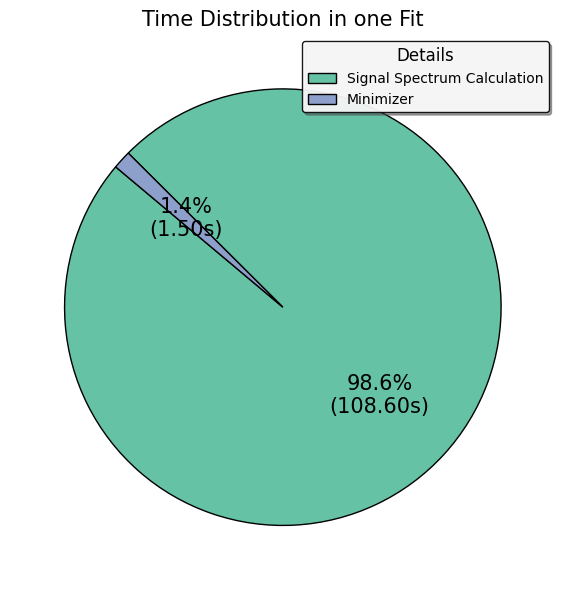
\includegraphics[width=0.55\textwidth]{Img/time_distribution_in_one_fit.png}
  \bicaption{单次拟合中各主要处理阶段的时间占比。谱计算（绿色）主导总耗时，而最小化器（紫色）仅占少量比例。}{Relative contributions of major processing stages in one fit. The signal spectrum calculation (green) dominates the runtime, whereas the minimizer (purple) accounts for only a minor share.}
  \label{fig:acc_time_distribution_in_one_fit}
\end{figure}

进一步对能谱计算任务进行细分（见图~\ref{fig:acc_time_distribution_in_signal_spectrum_calculation}），发现计算时间主要消耗于两项核心子任务：探测器响应矩阵的构建以及沉积能量谱的生成与映射。

\begin{figure}[htbp]
  \centering
  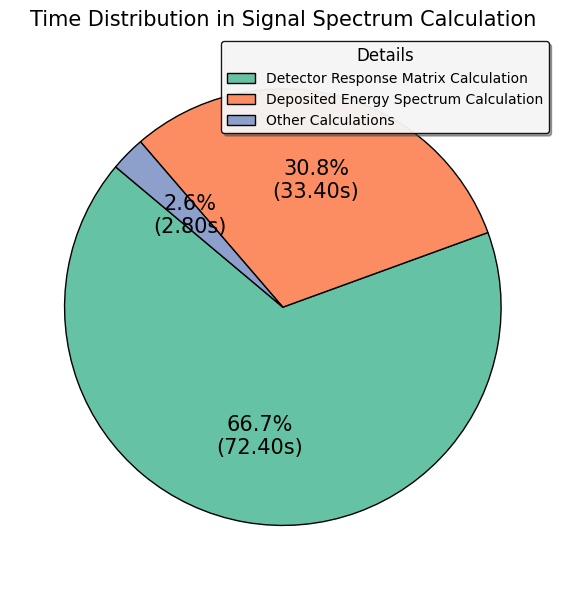
\includegraphics[width=0.55\textwidth]{Img/time_distribution_in_signal_spectrum_calculation.png}
  \bicaption{能谱计算内部的时间构成。探测器响应矩阵的计算（绿色）占多数，其次是沉积能量谱的生成（橙色），其余任务占比很小（蓝色）。}{Internal decomposition of the signal spectrum calculation. Most of the time is spent on the detector response matrix calculation (green), with additional contributions from the generation of the deposited energy spectrum (orange) and other minor tasks (blue).}
  \label{fig:acc_time_distribution_in_signal_spectrum_calculation}
\end{figure}

更细致的热点分析表明：
\begin{enumerate}
  \item \textbf{探测器响应矩阵计算}：在当前实现中，构造响应矩阵 \(R\) 需要对所有重建能量箱边界与可见能量采样点计算差值与归一化因子（大致对应一个 \(560\times5600\) 的减/除操作阵列），并对每个元素评估误差函数 \(\operatorname{erf}\) 以得到累积分布函数（CDF）。该过程伴随高强度的算术运算（Arithmetic Intensity）及大量特殊函数（误差函数 $\operatorname{erf}$）的调用。该环节耗时约 72.4 s，占谱计算总耗时的 66.7\%。         
  \item \textbf{沉积能谱计算}：这里的主要开销来自用微分散射截面（IBD mapping）矩阵将中微子能量映射到沉积能量的矩阵—向量乘法，在当前能量网格下，这等效于对约 $5600 \times 5600$ 维度的密集矩阵进行乘法运算，耗时约 33.4 s（占比 30.8\%）。
\end{enumerate}

基于上述剖析，本研究将优化重点放在两个热点之上，并制定相应的加速策略：
\begin{itemize}
  \item \textbf{响应矩阵加速}：对探测器响应矩阵计算采用分块构造，并可选地对 $\pm 6\sigma$ 区间进行截断，以减少误差函数 erf() 的无效计算。
  \item \textbf{IBD微分散射截面映射加速}：对 IBD 微分散射截面映射采用带状稀疏矩阵表示，利用其有限带宽特性采用稀疏乘法跳过大量零元素，从而降低内存与乘法开销。
\end{itemize}
此外，我们还引入了中间量缓存（caching）策略——对与物理参数无关且在多次拟合中重复使用的中间结果（例如响应矩阵的若干分块、固定的能量网格上的累积分布值等）进行缓存以避免重复评估。上述三类措施分别从减少特殊函数调用、降低矩阵运算复杂度与消除重复计算三方面切入，能够在不牺牲谱形精度的前提下，显著降低单次拟合的计算成本。


\section{加速策略实现与基准测试}
\label{sec:techniques}

\subsection{缓存技术}
\label{sec:caching}
在反应堆中微子能谱拟合中，往往伴随大量重复的矩阵运算与非线性变换——这些中间计算既占用 CPU 也带来频繁的 I/O。为降低重复计算开销、提高拟合与大规模 toy-MC 管线的整体吞吐量，我们在框架中引入了分层缓存机制（caching），以避免在参数估计和伪实验生成过程中对不必要的中间量反复求值。缓存策略主要在两个层面实施：

\textbf{静态量的预计算与常驻内存}

对于拟合过程中恒定不变的输入量，在拟合开始前一次性计算并加载到内存中。典型的静态量包括：

\begin{enumerate}
    \item 各裂变同位素的反中微子基准能谱 $\phi_i(E_{\bar{\nu}_e})$（如 ${}^{235}$U、${}^{238}$U、${}^{239}$Pu、${}^{241}$Pu）；
    \item IBD 的微分散射截面映射矩阵 $\sigma(E_{\bar{\nu}_e}\to E_{\rm dep})$；
    \item 探测器能量响应模型中的默认非线性响应曲线；
    \item 各类本底的谱形（如 Bi-Po214、宇宙线次级粒子、大气中微子、地球中微子、$^{13}$C($\alpha$,n)$^{16}$O 等）。
\end{enumerate}

将上述静态输入在拟合前预计算并常驻内存，一方面避免每次拟合或每次迭代时重复从磁盘加载，减少 I/O 开销；另一方面避免重复执行数值积分或插值，节省了大量 CPU 时间。

\paragraph{动态量的函数级复用（memoization）}
对于拟合过程中随参数变化、需要在每次迭代中更新的量（例如预测重建能量能谱、参数化能量非线性函数，或与响应矩阵及冗余参数组合相关的中间结果），其理论上需要逐次重新计算；但在实际拟合与大规模 toy-MC 中，常会出现\emph{相同输入反复出现}的情况。为避免重复求值，我们在函数层面引入缓存（memoization），实现上可直接使用 Python 标准库的 \texttt{functools.lru\_cache}（或等价的哈希缓存）。其核心思想是维护一个定长键值表：当相同参数的函数调用再次发生时，直接返回已缓存的结果而不进行数值计算。

\paragraph{数值实现注意事项}
对浮点参数而言，缓存命中要求参数的二进制表示（及其哈希）完全一致，因此默认情况下\textbf{不具备数值公差容忍}。工程实现中可通过以下方式提升命中率并控制误差：
\begin{itemize}
    \item 对浮点参数进行离散化/量化（quantization），例如按固定精度四舍五入后再参与哈希；
    \item 设计归一化的函数签名（统一单位与尺度、显式截断无关小数位），避免"数值等价输入"产生不同键值。
\end{itemize}

\paragraph{收益与可复用性}
函数级缓存对计算复杂且调用频繁的算子尤为有效，例如谱形卷积、矩阵乘法（或其分块子操作）以及误差函数 \(\operatorname{erf}\) 的批量评估。在广域参数扫描与 toy-MC 密集任务中，该策略可显著降低重复计算比例、提升整体吞吐量；基准测试表明，总拟合时间可降至约原来的三分之一（约 \(3\times\) 加速）。类似的缓存/预载策略在其他中微子分析框架中也已被验证有效，例如 GooStats 通过预载探测器响应网格实现了超过一个数量级的加速~\cite{Ding_2018}。本工作的缓存设计具有通用性，易于迁移到其它基于 forward-folded 能谱的实验分析，尤其适用于高维系统模型与大规模统计构造场景。

\subsection{微分散射截面矩阵的稀疏表示与响应矩阵分块优化}

\begin{figure}[htbp]  
    \centering  
    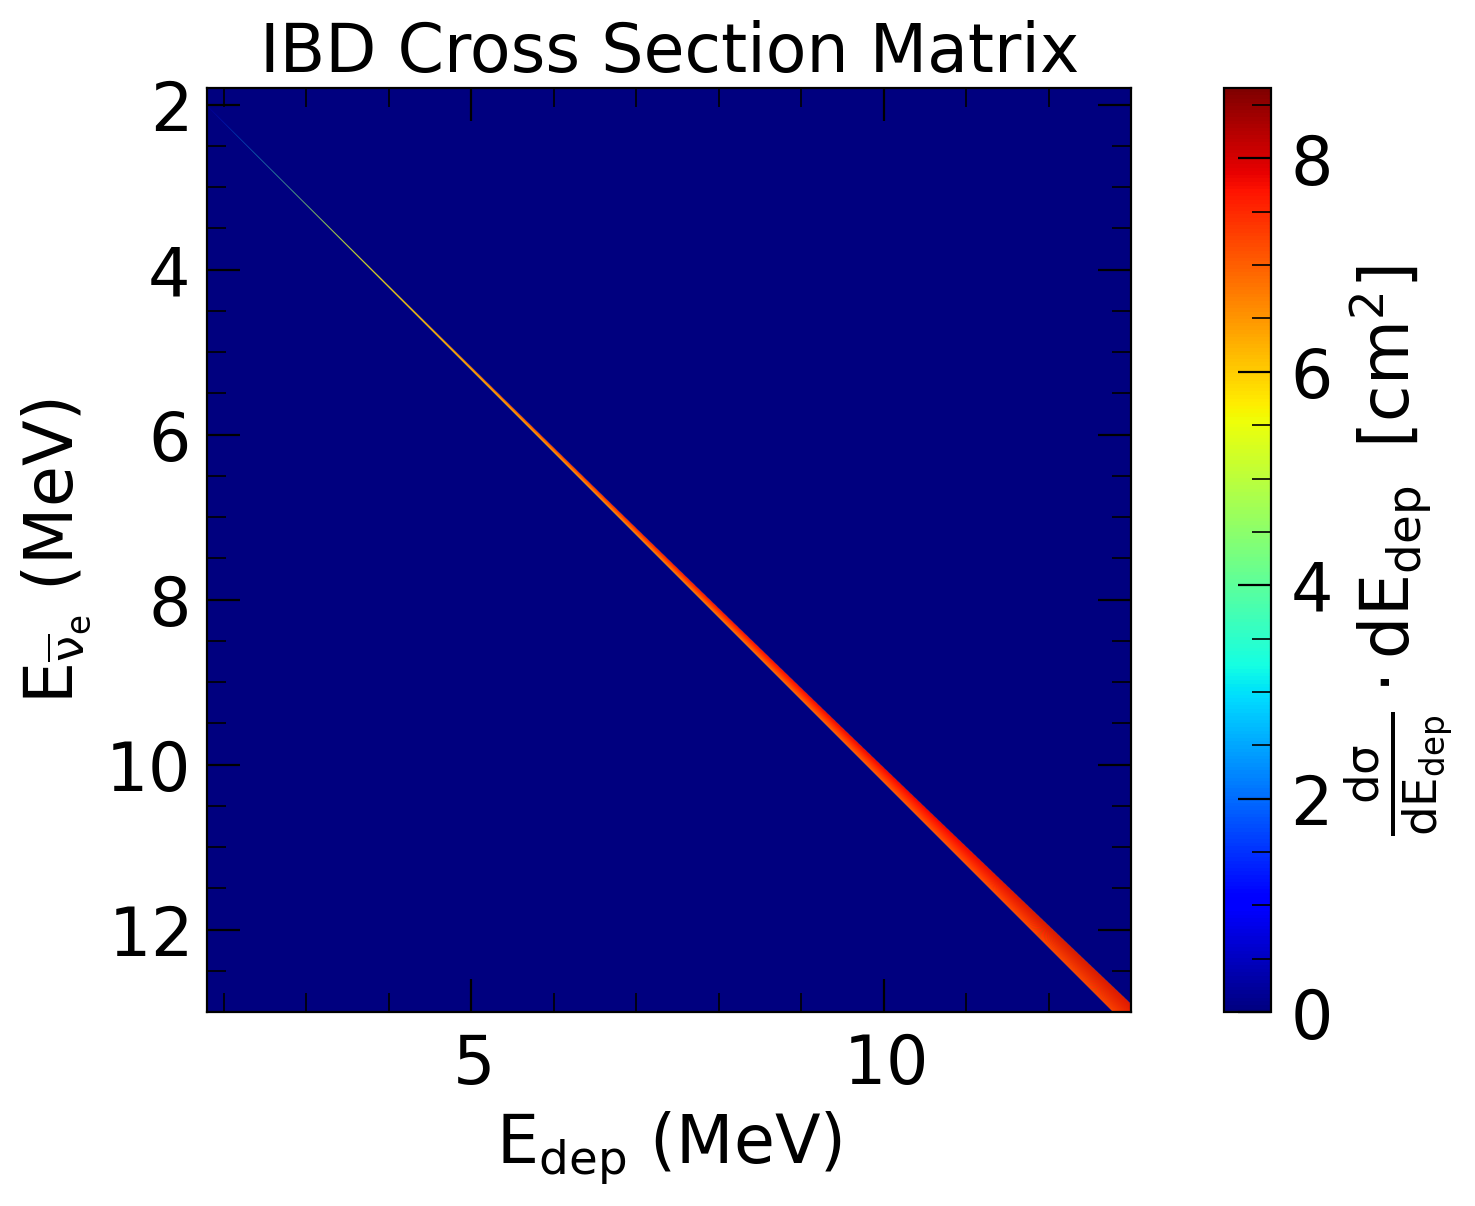
\includegraphics[width=0.55\textwidth]{Img/IBD_cross_matrix.png}  
    \bicaption{IBD 微分散射截面矩阵 $\dfrac{\mathrm{d}\sigma}{\mathrm{d}E_{\rm dep}}(E_{\rm dep},E_{\bar{\nu}_e})$ 的热力图（色标单位为 $10^{-44}$ cm$^2$ / 2 keV）。横轴为沉积能量 $E_{\rm dep}$（MeV），纵轴为入射反中微子能量 $E_{\bar{\nu}_e}$（MeV）；颜色越暖表示微分散射截面值越大。图中清晰可见主对角带，表明矩阵适合采用带状稀疏表示以加速谱的构造与拟合。}{Differential inverse beta-decay (IBD) cross-section matrix $\dfrac{\mathrm{d}\sigma}{\mathrm{d}E_{\rm dep}}(E_{\rm dep},E_{\bar{\nu}_e})$ is shown as a color map (color scale in units of $10^{-44}$ cm$^2$ per 2keV). The horizontal axis is the deposited energy $E_{\rm dep}$ (MeV) and the vertical axis is the incident antineutrino energy $E_{\bar{\nu}_e}$ (MeV); warmer colors denote larger differential cross-section values. This mapping is used to project theoretical neutrino-energy spectra into deposited-energy space for spectrum construction and fitting.}  
    \label{fig:sparse_cross_section}  
\end{figure}

在反应堆反电子中微子谱拟合中，从中微子能量 $E_{\bar{\nu}_e}$ 到沉积能量 $E_{\rm dep}$ 的映射由 IBD（逆贝塔衰变）微分散射截面控制，该映射可表示为二维响应矩阵 $M[i,j]$，其元素 $M_{ij}$ 表示入射能量为 $E_{\bar{\nu}_e,j}$ 的反中微子经 IBD 在沉积能量箱 $i$ 中产生信号的概率密度。受 IBD 动力学约束（尤其是正电子能量与发射角之间的耦合）影响，该矩阵呈现出明显的带状稀疏结构：非零元主要集中在主对角附近，满足近似关系

$$E_{\rm dep,i} \approx E_{\bar{\nu}_e,j} - \Delta,$$

其中 $\Delta\approx 0.8\ \mathrm{MeV}$ 包含了阈值与湮灭修正。该稀疏模式在图~\ref{fig:sparse_cross_section} 中有直观展示，主对角线附近有明显的带状结构。

鉴于大多数矩阵元素为零或接近零，我们采用 PyTorch 提供的稀疏存储格式（如 CSR/带状存储）来保存微分散射截面矩阵 $M$。稀疏格式只记录非零元素的位置与数值，从而显著降低内存占用并避免对零元的冗余计算。在谱生成与拟合过程中，响应矩阵 $M$ 与按振荡参数计算得到的中微子通量向量 $\boldsymbol{\phi}(E_{\bar{\nu}_e})$ 做乘法得到沉积能量谱 $S(E_{\rm dep})$。利用稀疏表示后，矩阵—向量乘法的计算复杂度可由 $O(N^2)$ 降为 $O(Nw)$，其中 $N$ 为能量格点数，$w$ 为带宽（非零元在对角带上的宽度），通常远小于 $N$，因此能获得显著的计算加速。

此外，稀疏表示在现代硬件（包括多核 CPU 与 GPU）上通常有更好的缓存局部性和更高的内存带宽效率，从而进一步提升并行计算中的吞吐量。我们的基准测试表明，在 Intel Xeon Gold 6338 平台上，不牺牲数值精度的前提下，采用稀疏表示与稀疏乘法可使微分散射截面映射步骤的计算时间缩短约 4 倍，成为整个加速管线中的关键组成部分。

类似的思想也被 ReMU 等框架采用：仅保留含非零元的行并结合高效的线性代数操作，以提升能谱构造效率~\cite{Koch2019}。总体而言，充分利用微分散射截面矩阵的稀疏性不仅能显著减少存储与计算开销，而且对中微子能谱拟合在高精度、低统计或大规模 toy-MC 分析下的可扩展性与性能影响深远。

\paragraph*{探测器响应矩阵的分块构造}\mbox{}\\
探测器响应矩阵用于将粒子在闪烁体中沉积的真实能量映射为对应的重建能量分布。矩阵的每个元素表示某一沉积能量落入某一重建能量箱的概率。在传统实现中，该响应矩阵通常为一个二维数组，尺寸约为 $560\times5600$：560 个重建能量箱对应横轴，5600 个沉积能量箱对应纵轴。构造该矩阵时，往往逐元素计算——先计算待测沉积能量与重建能量边界的差值，再除以标准差并对误差函数 $\operatorname{erf}$ 求值以得到累积分布函数（CDF），最后取相邻 CDF 的差值得到每个元素的概率。这种按元素计算的实现代价很高：一方面 $\operatorname{erf}$ 等特殊函数本身计算开销大；另一方面若一次性构造整个矩阵，则需在内存中保存大量中间结果，导致显著的内存占用与数据搬运开销。总体而言，逐元素一次性构造的方法在计算复杂度和内存消耗上都存在严重瓶颈。

为降低计算与内存负担，本工作采用了分块（block）处理策略：将 $560\times5600$ 的矩阵沿列方向切分为若干小的子块\cite{Lam1991}，并对每一子块逐个进行计算与累积。具体做法为：每次仅取出一个列区间内的沉积能量数据，在该区间上计算对应的重建能量概率分布；完成后将该子块的结果累加或拼接到最终的响应矩阵中，然后释放该子块的中间数据再继续处理下一个子块。这样一来，计算就被约束在较小的数据块上，有利于缓存（cache）重用并显著减少内存间的数据搬运；由于始终只保留当前子块的中间结果，无需为整个大矩阵分配峰值内存，从而大幅降低峰值内存使用与内存带宽压力。


分块计算方法在实践中带来了可观的性能提升。块宽的最优取值通过在测试平台（Intel Xeon Gold 6338）上对若干候选值（128、256、512、1024）进行基准测试确定：块宽 512 时耗时最短，这与其硬件对齐特性一致——512 为 2 的幂次（$2^9$），与 CPU 缓存行（cache line，通常 64 字节）对齐良好；512 个 float32 元素仅占 2 KB，可完整驻留于 L1 数据缓存（32 KB），从而最大化缓存命中率。块宽过小（如 128）时分块开销相对增大，过大（如 1024）时数据超出 L1 缓存导致命中率下降，故 512 为该平台上的经验最优值。在块宽设置为 512 时，探测器响应矩阵的构造时间从约 55 ms 降至约 27 ms，约为 $2\times$ 的加速比。该方法之所以有效，主要在于它充分利用了数据局部性（data locality），使得对 $\operatorname{erf}$ 等数值操作的调用更容易命中高速缓存，减少了重复 I/O 与索引开销，从而降低了整体运行时间与资源消耗。

\subsection{加速结果}
本节评估在中微子能谱拟合中应用各类优化技术所带来的性能提升。所有基准测试均在同一台服务器上进行，测试平台为 Intel Xeon Gold 6338（2.00 GHz）。我们考察了三类主要的加速策略：

\begin{enumerate}  
\item 引入缓存技术（caching）；  
\item 使用稀疏表示存储微分散射截面矩阵；  
\item 采用分块计算优化探测器响应矩阵的构造与乘法。  
\end{enumerate}

对各项优化所获得的加速比进行了逐项测试。将探测器响应元素的计算限制在 $\pm6\sigma$ 范围内（截断高斯尾）在 NumPy 实现上可以带来约 $1.5\times$ 的加速，但在结合其它基于 PyTorch 的优化后，其增益可忽略不计，因此未在最终实现中启用此截断策略。缓存技术贡献了约 $3\times$ 的加速；将微分散射截面矩阵以稀疏格式存储带来了约 $1.5\times$ 的加速；而分块乘法/分块构造则再带来大约 $1.5\times$ 的加速。综合应用所有优化后，单次拟合的总耗时从原始的 $110.1\ \mathrm{s}$ 降至 $15.2\ \mathrm{s}$，总体约达到 $\approx 7\times$ 的加速。该结果见图~\ref{fig:fit_per_t_opt}。

\begin{figure}[htbp]  
\centering  
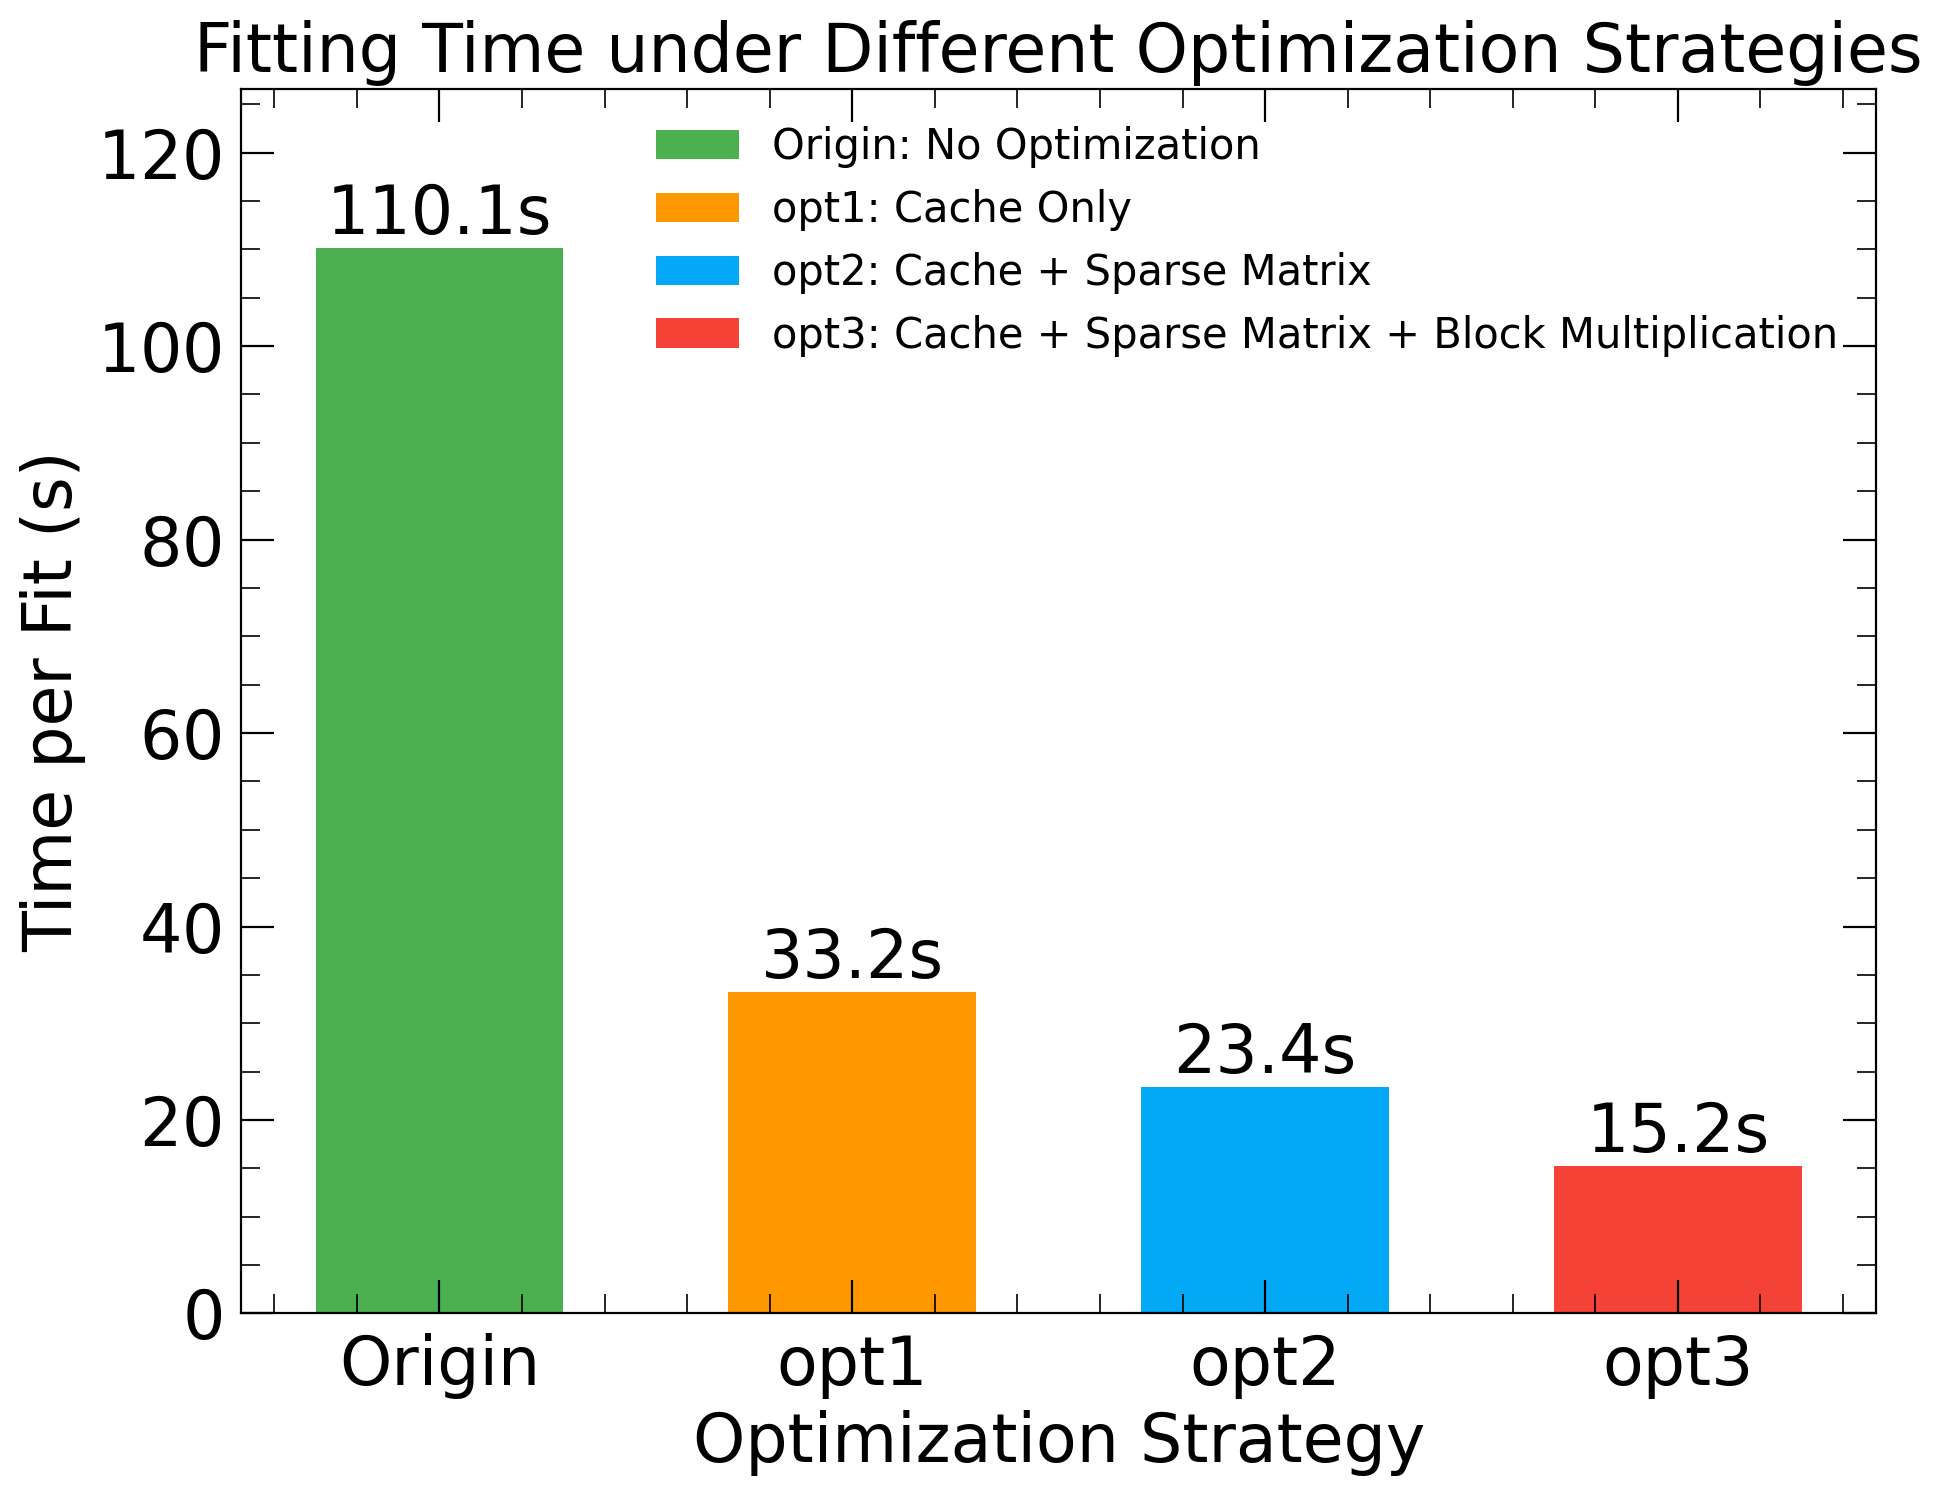
\includegraphics[width=0.6\textwidth]{Img/fitting_time_under_different_optimization_strategies.png}  
\bicaption{不同优化策略下单次拟合平均耗时比较。横坐标依次为：未经优化的基线实现（\textit{Origin}）、仅启用缓存（\textit{opt1}）、缓存 + 微分散射截面稀疏表示（\textit{opt2}）、缓存 + 稀疏表示 + 分块乘法（\textit{opt3}）。纵坐标为单次拟合的平均壁钟时间（秒）。柱状图展示了随着逐步应用优化策略，运行时间的逐级下降；其中 \textit{opt3} 达到最短的拟合时间。}{Comparison of average fitting time per fit under different optimization strategies. The horizontal axis lists the tested strategies: the baseline without optimization (\textit{Origin}), caching only (\textit{opt1}), caching with sparse matrix representation (\textit{opt2}), and caching with sparse matrix representation plus block multiplication (\textit{opt3}). The vertical axis shows the average wall-clock time in seconds required for a single fit. The bars illustrate the progressive reduction in runtime as successive optimizations are applied, with \textit{opt3} achieving the shortest fitting time.}  
\label{fig:fit_per_t_opt}  
\end{figure}

图~\ref{fig:computation_time_comparison_before_after_acceleration} 显示了针对关键模块的定量对比：在定点优化后，整体拟合性能显著提升。用于计算期望信号谱的时间由原来的 $108.6\ \mathrm{s}$ 降至 $14.3\ \mathrm{s}$，约为 $8\times$ 的加速。在谱计算内部的两大热点上，探测器响应矩阵的构造时间从 $72.4\ \mathrm{s}$ 缩短到 $8.1\ \mathrm{s}$（约 $9\times$ 加速），而沉积能量谱的计算（包括微分散射截面映射与矩阵乘法）则从 $33.4\ \mathrm{s}$ 缩短到 $5.0\ \mathrm{s}$（约 $6\times$ 加速）。其余次要任务时间变化甚微，不影响总体结论。

\begin{figure}[htbp]  
\centering  
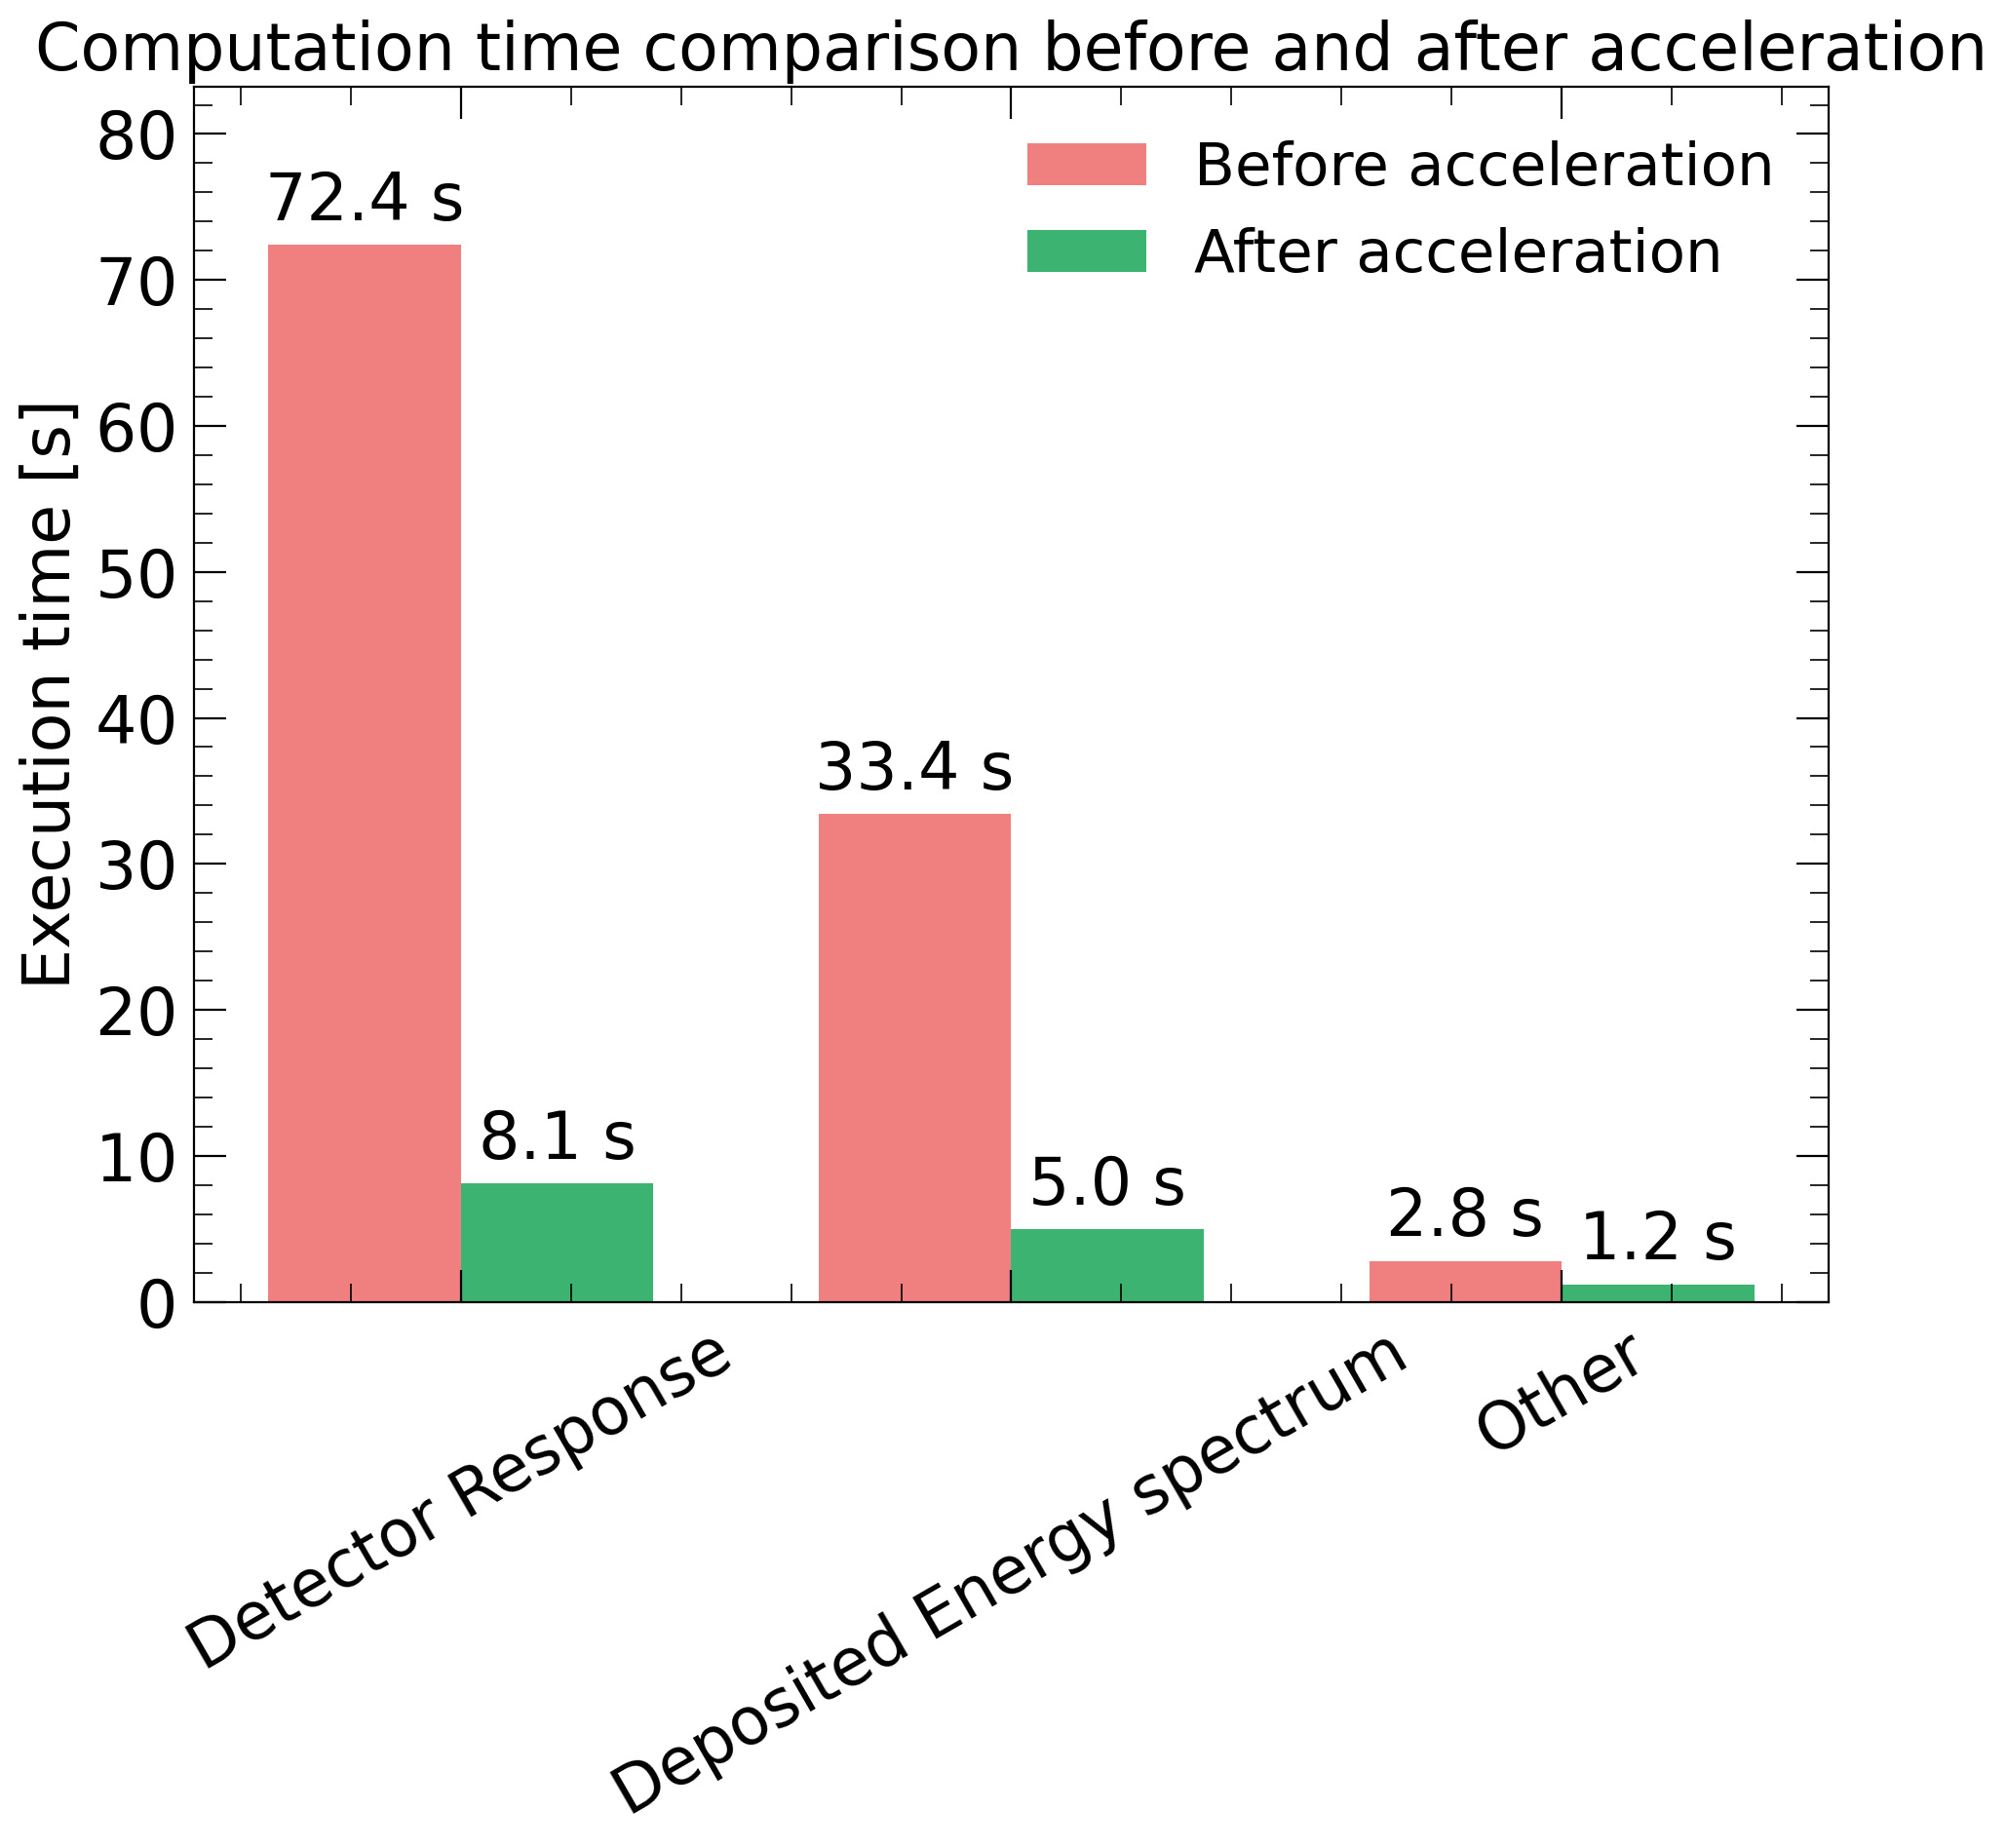
\includegraphics[width=0.6\textwidth]{Img/computation_time_comparison_before_after_acceleration.png}  
\bicaption{主要模块在应用加速技术前后的计算时间对比。图中显示探测器响应矩阵与沉积能量谱计算这两项主导性任务在加速后均获得显著缩短，从而推动整体拟合耗时的大幅下降。}{Computation-time comparison of major modules before and after acceleration. The dominant tasks—detector response matrix construction and deposited-energy spectrum calculation—are significantly reduced after optimization, leading to a large decrease in the overall fit time.}  
\label{fig:computation_time_comparison_before_after_acceleration}  
\end{figure}

综上所述，通过缓存、稀疏化与分块处理三类互补的工程与算法优化措施，我们在不牺牲拟合精度的前提下，实现了对能谱拟合的显著加速。该性能提升将使得原本因计算代价难以承受的大规模 Feldman–Cousins 覆盖性构造与广域 toy-MC 扫描变为可行，从而支持更严格的频率学置信区间验证与更全面的参数空间探索。

\subsection{能谱分箱对拟合耗时的影响}  
\label{sec:bin}

我们还研究了不同重建能量分箱数对总体拟合耗时的影响。固定重建能量观测区间为 $[0.8,\,12.0]$ MeV，分别将该区间等距划分为 $N_{\rm bin}=560,\;280,\;140,\;70,\;35$ 个箱，并在相同的优化策略下进行基准测试。图~\ref{fig:fit_time_per_bins} 给出了在若干优化配置下，单次完整拟合耗时随直方图 bin 宽变化的依赖关系。可以看到，在所有测试情形下，随着 bin 宽增大（即箱数减少），单次拟合耗时单调下降。其根本原因是：增大 bin 宽会减少重建能量能谱的箱数 $M$，从而缩小探测器响应矩阵的维度，降低每次似然评估所需的计算量。

我们考察的优化策略包括：缓存（caching）、微分散射截面稀疏（CSR）表示、以及分块（tiled）乘法/分块构造。缓存与稀疏表示在整个 bin 宽范围内均能稳定带来加速；而分块乘法在箱数较多（bin 宽较细、矩阵尺寸最大）时能显著提升性能，但当 bin 较粗时分块带来的优势会减小甚至消失。

在反应堆反中微子拟合中，探测器响应矩阵 $R$ 的构造与应用是主要的计算瓶颈之一。设 $R$ 的尺寸为 $M\times N$，其中 $M$ 为重建能量箱数，$N$ 为沉积能量箱数。每个矩阵元 $R_{ij}$ 都需通过高斯积分（误差函数 $\operatorname{erf}$）评估以得到相应的概率，因此直接构造完整矩阵的标量运算量可近似表示为

$$\text{Cost}_{\text{full}} \propto C \times M \times N,$$

其中常数 $C$ 表示构造每个元素所需的代价（包括若干次浮点减法、除法及一次 $\operatorname{erf}$ 计算）。忽略常数因子，总体计算复杂度规模为

$$T_{\text{full}}=\mathcal{O}(M\cdot N).$$

当增大重建或沉积能量能谱的 bin 宽（即降低分辨率）时，$M$ 或 $N$ 会相应下降；例如在固定区间 $[E_{\min},E_{\max}]$ 下，若将 bin 宽加倍，则箱数 $M$ 减半，总体计算量按线性比例缩减。

然而，当矩阵尺寸下降到足够小的阈值后，每个计算块已经足以完全驻留在 CPU 的缓存中，原先分块处理带来的缓存局部性优势将消失。同时，分块处理本身存在固定开销（函数调用、内存对齐与切片等），这些固定开销在单块计算量变小后会变得相对显著，从而抵消原先因改进局部性而得到的性能提升。因此，若箱数继续减小至某一临界点（即 bin 足够稀疏），分块方法的实际加速效应会趋近于零。

图中还标注了若干采样点的拟合迭代次数（所示点的注记），可见在不同 bin 宽下拟合器的迭代次数变化很小，这表明分箱选择主要影响的是每次迭代的计算成本，而不是最小化算法的收敛行为。

综上所述，较细的分箱会显著增大探测器响应矩阵的规模和每次迭代的计算量，使得采用先进的加速策略（如缓存、稀疏化与分块化）成为保持可接受拟合时间的必要手段；而对于较粗的分箱，矩阵尺寸天然变小，单次计算成本降低，使得分块矩阵乘法等性能优化的效果下降。

\begin{figure}[htbp]  
\centering  
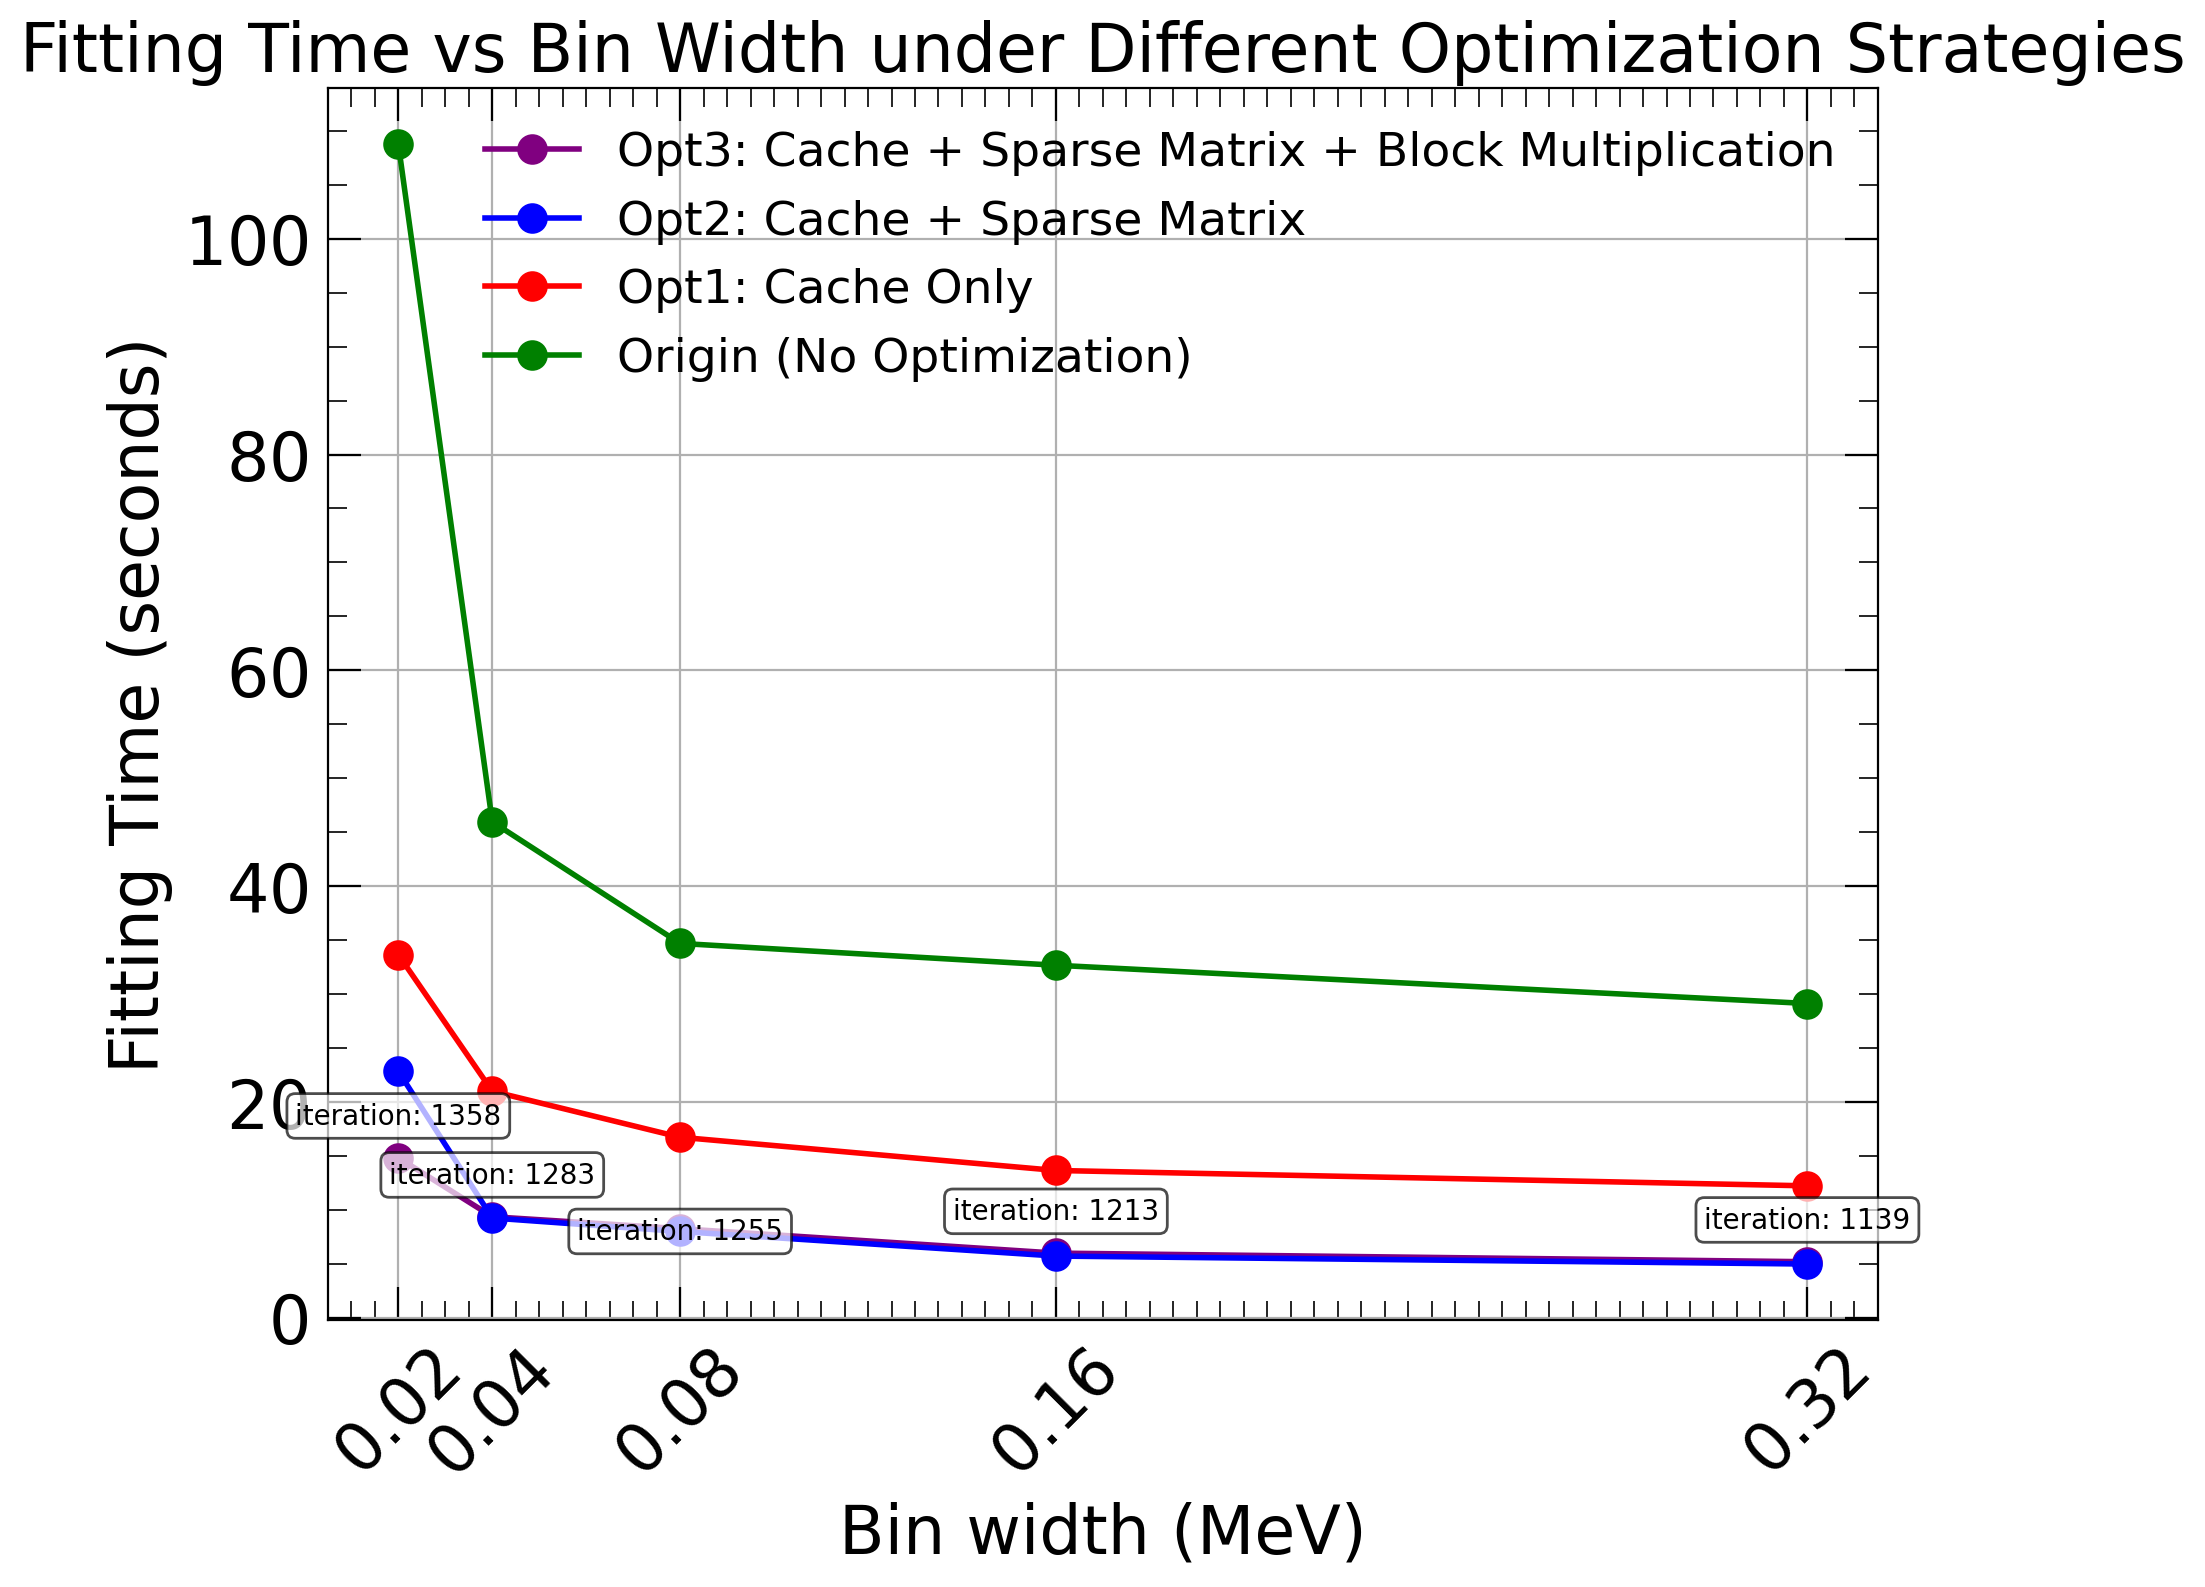
\includegraphics[width=0.6\textwidth]{Img/fitting_time_vs_bin_width.png}  
\bicaption{单次完整拟合耗时随重建能量能谱 bin 宽的变化。横轴为重建能量能谱直方图的 bin 宽（MeV）；纵轴为单次完整拟合的时间（秒）。曲线对应不同的优化配置：绿色 — 基线（无优化）；红色 — 仅缓存；蓝色 — 缓存 + 稀疏（CSR）存储；品红色 — 缓存 + 稀疏 + 分块（tiled）乘法。每个点均在相同的能量区间 $[0.8,\,12.0]$ MeV 下通过不同等距箱数计算得到。}{Fitting time as a function of reconstruction-bin width. The horizontal axis shows the bin width of the reconstructed-energy histogram (MeV); the vertical axis gives the total wall-clock fitting time (s) for a single full fit. Curves correspond to different optimization configurations: green — baseline (no optimization); red — caching only; blue — caching + sparse (CSR) matrix storage; magenta — caching + sparse matrix + block (tiled) matrix multiplication. Each point was obtained for the same reconstructed-energy interval ([0.8, 12.0] MeV) but with different numbers of uniform bins (equivalently different bin widths).}  
\label{fig:fit_time_per_bins}  
\end{figure}

\section{本章小结}
\label{sec:ch3_summary}
本章内容提出的多项加速技术在保证数值精度的前提下，显著提升了反应堆反中微子能谱拟合的计算效率。具体而言：

首先，通过缓存（caching）策略将拟合过程中频繁重复出现的中间计算结果保存并复用，避免了大量冗余计算。基准测试表明，仅启用缓存即可将拟合速度提高约 $3\times$。

其次，充分利用微分散射截面矩阵与响应矩阵的带状稀疏性，将这类矩阵以压缩稀疏格式（如 CSR）存储，并仅对非零元执行计算，从而大幅减少乘加运算与内存访问。我们的测试显示，这一稀疏化处理带来了约 $1.5\times$ 的加速。

再次，通过对探测器响应矩阵采用分块（blocked / tiled）乘法与逐块构造的方法，可改善数据局部性并降低内存搬运开销。该方法在我们的实现中同样贡献了约 $1.5\times$ 的加速。

将上述三类技术组合后，相较于未经优化的实现，总体拟合耗时在本测试环境下缩短了约 $7\times$。

我们还量化了重建能量分箱对计算耗时的影响。增大 bin 宽（即减少箱数）会直接缩小响应矩阵的维度，从而使每次似然/χ²评估的计算成本按矩阵规模近似线性下降；在我们的测试中，最小化器迭代次数基本保持不变，因此总耗时主要受每次迭代的计算代价驱动。由此可见，在分辨率与计算开销之间存在明显的权衡：极细的分箱会增加矩阵规模，这时分块乘法的加速效果最优；而缓存与稀疏存储在广泛的分箱设置下均能提供稳健的加速效果。

总体而言，本工作所采用的缓存、稀疏化与分块等互补性优化措施，大幅降低了重建能量能谱拟合的计算代价，构建了一个高效且可扩展的前向折叠（forward-folding）加速框架。该方法对当前与未来的中微子实验（例如 JUNO、Hyper-Kamiokande、DUNE 等）具有广泛适用性，有助于开启更大规模的 toy-MC 研究、更快速的参数扫描以及更可行的频率学置信带（Feldman–Cousins）构造。


